\documentclass{article}
\usepackage{graphicx}
\usepackage{amsmath}
\usepackage[margin=1in]{geometry}

\author{Michael Bentley}
\title{Project 4: CasADi playing}
\date{05 Feb 2019}

\begin{document}
\maketitle

CasADi is a symbolic framework for nonlinear optimization and algorithmic
differentiation.
%
Here we use CasADi not as intended.
%
We are using it as a gateway to utilizing the nonlinear optimization solvers it
employs.
%
However, CasADi is targeted to solving optimal control problems.


\section{Reaching Desired Task Space Positions}

This is all about reaching the goal.

\subsection{}

\begin{figure}
  \centering
  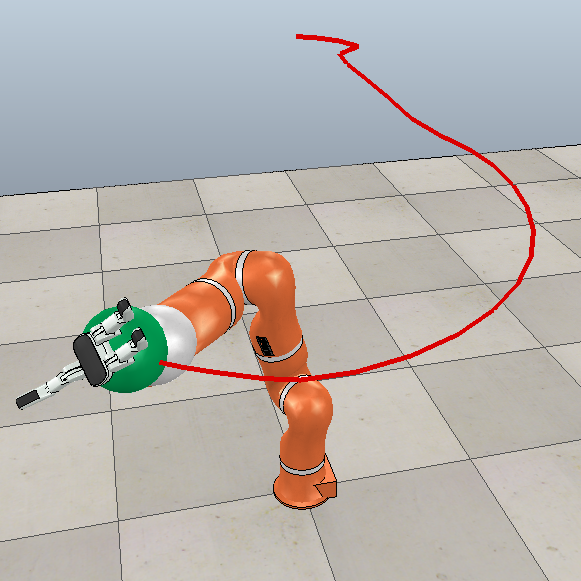
\includegraphics[width=.3\textwidth]{images/p1-1-1.png} \hspace{1em}
  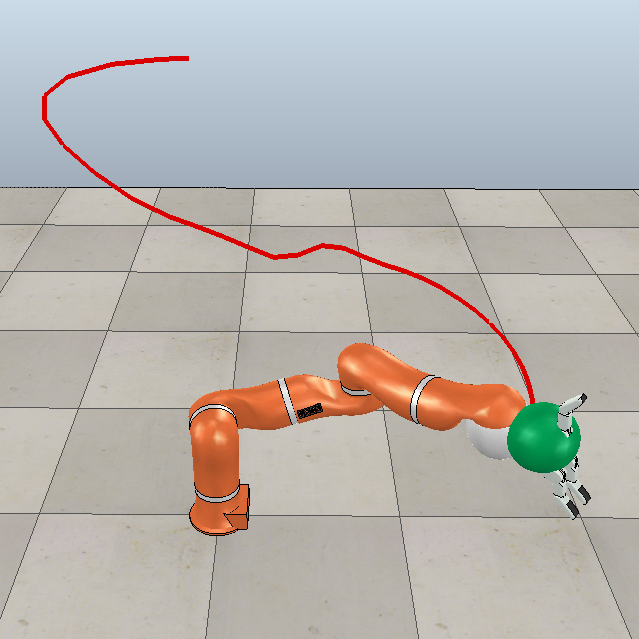
\includegraphics[width=.3\textwidth]{images/p1-1-2.png} \hspace{1em}
  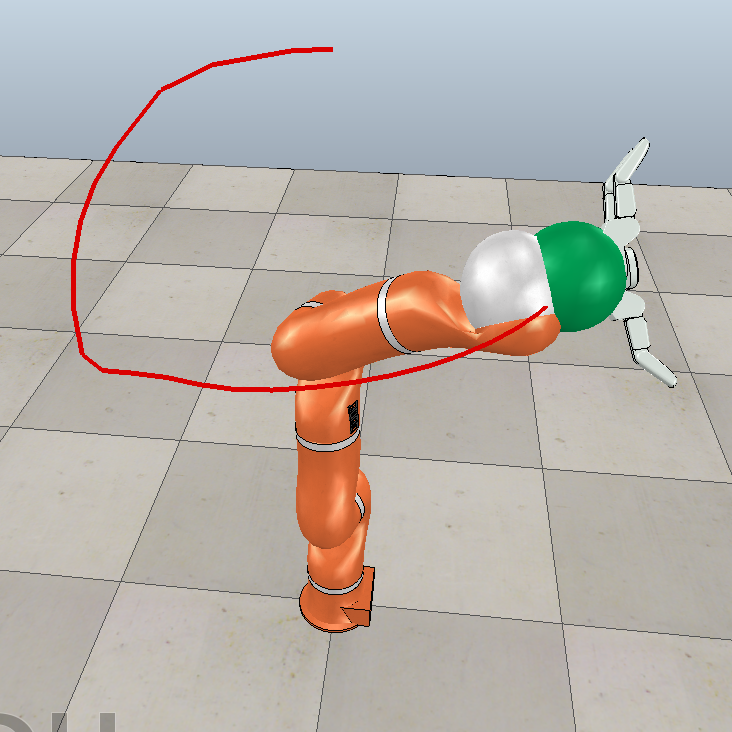
\includegraphics[width=.3\textwidth]{images/p1-1-3.png}
  \caption{
    Screenshots of three executions of problem 1.1 using randomly generated
    goal locations.
    }
  \label{fig:p1.1-screenshots}
\end{figure}

We are to implement the following optimization problem:

\begin{align*}
  \min_{\vec{\theta}}
    &
      \sum_{t = 1}^T
      ||
      FK(\vec{\theta}_t) - \vec{x}_g
      ||^2_2
  \\
  \text{s.t.}
    &
      \vec{\theta}_{lower}
        \leq
      \vec{\theta}_t
        \leq
      \vec{\theta}_{upper}
  \\
    &
      t = 1, \ldots, T.
\end{align*}

This was implemented and run three times.
%
In Figure~\ref{fig:p1.1-screenshots}, we see the screenshots after the three
executions with randomly generated goal locations.

\end{document}
